\pgfdeclaredecoration{penciline}{initial}{
    \state{initial}[width=+\pgfdecoratedinputsegmentremainingdistance,auto corner on length=1mm,]{
        \pgfpathcurveto%
        {% From
            \pgfqpoint{\pgfdecoratedinputsegmentremainingdistance}
                            {\pgfdecorationsegmentamplitude}
        }
        {%  Control 1
        \pgfmathrand
        \pgfpointadd{\pgfqpoint{\pgfdecoratedinputsegmentremainingdistance}{0pt}}
                        {\pgfqpoint{-\pgfdecorationsegmentaspect\pgfdecoratedinputsegmentremainingdistance}%
                                        {\pgfmathresult\pgfdecorationsegmentamplitude}
                        }
        }
        {%TO 
        \pgfpointadd{\pgfpointdecoratedinputsegmentlast}{\pgfpoint{1pt}{1pt}}
        }
    }
    \state{final}{}
}
\newsavebox{\NameBox}
\newsavebox{\SubjectsSmallBox}
\newsavebox{\SubjectsMediumBox}
\newsavebox{\SubjectsBigBox}
\newsavebox{\SubjectsGiantBox}

\newcommand{\updateNameBox}{
    \savebox{\NameBox}{
      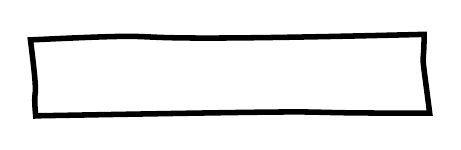
\begin{tikzpicture}[decoration=penciline]
        \node[decorate,draw, minimum height=1cm, minimum width=5cm, line width=2pt] {};
      \end{tikzpicture}
    }
}
\newcommand{\updateSubjectsSmallBox}{
    \savebox{\SubjectsSmallBox}{
      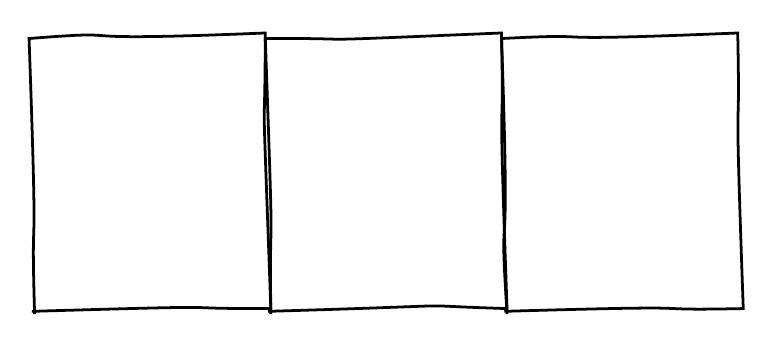
\begin{tikzpicture}[decoration=penciline]
        \node[decorate,draw, minimum height=3.5cm, minimum width=3cm, line width=1pt] {};
        \node[decorate,draw, minimum height=3.5cm, minimum width=3cm, line width=1pt,xshift=3cm] {};
        \node[decorate,draw, minimum height=3.5cm, minimum width=3cm, line width=1pt,xshift=6cm] {};
      \end{tikzpicture}
    }
}
\newcommand{\updateSubjectsMediumBox}{
    \savebox{\SubjectsMediumBox}{
      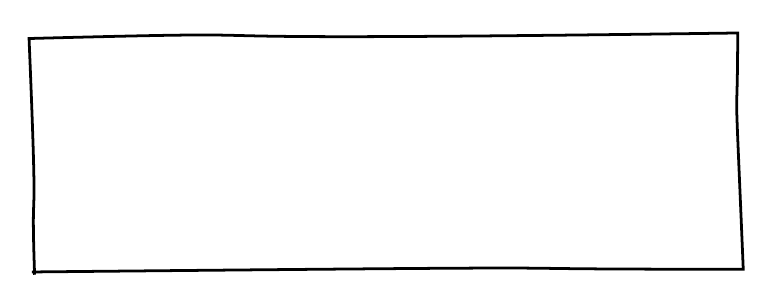
\begin{tikzpicture}[decoration=penciline]
        \node[decorate,draw, minimum height=3cm, minimum width=9cm, line width=1pt] {};
      \end{tikzpicture}
    }
}
\newcommand{\updateSubjectsBigBox}{
    \savebox{\SubjectsBigBox}{
      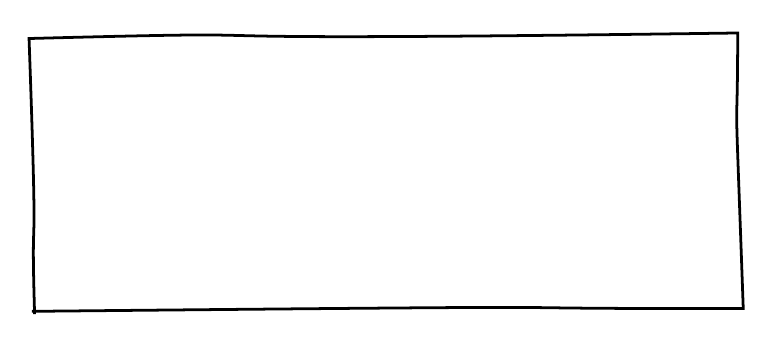
\begin{tikzpicture}[decoration=penciline]
        \node[decorate,draw, minimum height=3.5cm, minimum width=9cm, line width=1pt] {};
      \end{tikzpicture}
    }
}
\newcommand{\updateSubjectsGiantBox}{
    \savebox{\SubjectsGiantBox}{
      \begin{tikzpicture}[decoration=penciline]
        \node[decorate,draw, minimum height=11cm, minimum width=9cm, line width=1pt] {};
      \end{tikzpicture}
    }
}

\def\Step{0.25}  %% separation between dots
\def\Size{0.1pt}    %% radius of the dot

\newsavebox{\PaperPaternbox}
\sbox{\PaperPaternbox}{
\begin{tikzpicture}[remember picture]
    \foreach \y in {1,2,...,60}{
        \foreach \x in {1,2,...,60}
          \draw[fill=black,opacity=0.3,shift={(\Step*\x cm,\Step*\y cm)}] (0,) circle[radius=\Size];
    }
\end{tikzpicture}
}
